\section{Autonomy and Safety}
\label{sec:local}

%% This paper focuses on allowing ASes to autonomously and locally
%% determine their routing policies.  This is inherent in the current BGP
%% protocol: each provider independently sets its own routing policy, and
%% no global verification is performed on the resulting choices of
%% rankings and filters.  This is a feature that is desirable in any
%% large scale protocol, and thus we restrict attention to protocol
%% designs where providers are allowed to choose their rankings
%% locally.  

In this section, we determine necessary and sufficient constraints on
the allowable classes of rankings, such that if each AS autonomously
sets its ranking while filtering is unrestricted,
the protocol is guaranteed to be safe.  
%We use
%the static concepts of dispute rings and dispute wheels to simplify
%checking safety, a dynamic property.  Thus,
We do so by characterizing whether a routing system
where rankings are independently specified by each AS can induce
either a dispute ring or a dispute wheel.

%As previously discussed, we want to focus on protocols that respect
%autonomy.  
Any protocol's configurable parameters implicitly constrain
the rankings ASes can express.  For example, in BGP, the set of
protocol parameters is rich enough to allow providers to express
essentially any possible ranking over paths.  
%We restrict attention
%to protocols where these constraints respect the ability of each AS to
%set rankings independently.  
In Section \ref{ssec:local}, we
axiomatically formulate two properties that should be satisfied by any
protocol that respects autonomy: {\em permutation invariance} and {\em
scale invariance}.  The first requires the rankings allowed by the
protocol to be independent of node labeling, while the second requires
the allowed rankings to scale gracefully as nodes are added to the
system.  We abstract protocols satisfying these two conditions using
the notion of an {\em autonomous ranking constraint} (ARC) function;
such a function takes the ranking of a single AS as input, and accepts it if
that ranking is allowed by the protocol.  Observe that {\em any}
protocol that respects the ability of ASes to autonomously choose
rankings can be represented by a corresponding ARC function.

In Section \ref{ssec:localex}, we give two examples of such
functions: the shortest hop count ARC function (which only accepts
rankings where shorter paths are preferred to longer paths), and the
next-hop ARC function (which only accepts next hop rankings).  We then
determine the class of ARC functions such that, as long as each
node independently chooses an acceptable ranking, the resulting
{\em global} routing system will be safe under
filtering.  In Section~\ref{ssec:localresults},
we show that the only ARC functions that are safe under filtering are
nearly equivalent to the shortest hop count ARC function.

\subsection{ARC Functions}
\label{ssec:local}

In this section, we define an {\em autonomous ranking constraint}
(ARC) function, which serves as an abstraction of the protocol's
constraints on allowed rankings over routes.  We start by defining a
local ranking constraint (RC) function, which takes as input the ranking of
a single AS $i$, $\prec_i^N$ and determines whether that 
ranking is allowable.

\begin{defn}[Local RC function]
Given $N$ nodes, a {\em local ranking constraint (RC) function}
$\pi(\prec_i)$ takes as input the ranking of a single AS $i$ over all
paths in $\P_i^N$, and returns ``accept'' if $\prec_i$ is allowed by
$\pi$, and returns ``reject'' otherwise.  If $\pi(\prec_i) =$
``accept'', we will say that $\prec_i$ is $\pi$-accepted.  If we are
given a routing system $(N, \prec_1, \ldots, \prec_N, \F_1, \ldots,
\F_N)$ where each $\prec_i$ is $\pi$-accepted, we will say the routing
system is $\pi$-accepted.
\end{defn}

Because we are restricting attention to protocols that respect the
ability of ASes to choose rankings autonomously, a first condition
that must be satisfied is that constraints on rankings should be
``local'': that is, an AS should not face constraints on allowable
rankings due to the rankings chosen by other ASes.  For this reason,
{\em local} RC functions act only on the ranking of a single AS.  More
generally, protocols might place system-wide constraints on the vector
of rankings chosen by all ASes; such protocols should be represented
by ``global'' RC functions.  Of course, such protocols do not
respect autonomy, and so we do not consider them here.

%A local RC function formalizes the notion that any protocol inherently
%constrains the ranking an AS can express.  Note that local RC functions act
%only on the rankings of a single AS; this is natural given that we are
%only modeling protocols that respect the ability of ASes to choose
%rankings autonomously.

We now define two natural conditions any local RC function that preserves
autonomy should satisfy.  First, the local RC function's conditions
on rankings should provide consistent answers to different ASes,
regardless of the {\em labeling} of the ASes. That is, for the
local RC function to preserve uniformity, each AS should be subject to
the same constraints on routing policies, and those constraints should
not depend on the particular assignment of AS numbers to ASes.  For
example, suppose the routing system consists of three ASes, and AS $1$
has an accepted ranking where it prefers $1 2 3 0$ over $1 2 0$, and
$1 2 0$ over $1 0$.  Then we expect the same ranking should be
accepted, even if the labels of nodes are {\em permuted}.  For
example, suppose we permute the node labels that $1 \to 2$, $2 \to 3$,
and $3 \to 1$.  Then node $2$ should also have an accepted ranking
where it prefers $2 3 1 0$ over $2 3 0$, and $2 3 0$ over $2 0$ (because
$2310$, $230$, and $20$ are the new paths that result after applying
the permutation to $1230$, $120$, and $10$, respectively).  If this
property were not satisfied, then the set of accepted rankings
determined by a local RC function would depend on the global assignment of AS
numbers to nodes, not on the characteristics of the individual rankings themselves.
We call this notion {\em permutation invariance}; to define it
precisely, we must proceed through a sequence of definitions, starting
with {\em path permutation}.

\begin{defn}[Path permutation]
Given $N$ nodes, let $\sigma$ be a permutation of the nodes
$1,\ldots,N$.  Then $\sigma$ induces a {\em path permutation} on any
path $P = i i_1 i_2 \ldots i_m j$ from $i$ to $j$, yielding a new path
$\sigma(P) = \sigma(i) \sigma(i_1) \sigma(i_2) \ldots \sigma(i_m) \sigma(j)$
from $\sigma(i)$ to $\sigma(j)$.  We always define $\sigma(0) = 0$.
\end{defn}

%% A path permutation defines a relabelling of nodes in the routing system,
%% but, for a routing system to be equivalent (except for node labelling
%% after a permutation is applied), the rankings must also be permuted
%% in a way that is consistent with the relabelling of nodes.  For this
%% purpose, we define a ranking permutation.

\begin{defn}[Ranking permutation]
Given $N$ nodes, let $\sigma$ be a permutation of the nodes
$1,\ldots,N$.  Then $\sigma$ induces a {\em ranking permutation} on
a ranking $\prec_i$ for node $i$ over the paths in
$\P_i^N$, yielding a new ranking $\sigma(\prec_i)$ over
the paths in $\P_{\sigma(i)}^N$, as follows: 
If $P_1, P_2 \in \P_i^N$, and $P_1 \prec_i P_2$, then $\sigma(P_1) 
\sigma(\prec_i) \sigma(P_2)$ (where $\sigma(P_i)$ is the path
permutation of path $P_i$ under $\sigma$).
\end{defn}

Note that a
permutation does not modify the routing system any substantive way, except to {\em
relabel} the nodes, and to relabel the paths and rankings and in a
way that is consistent with the relabeling of nodes.

\begin{defn}[Permutation invariance]
A local RC function $\pi$ is {\em permutation invariant} if, given $N$ and a
ranking $\prec_i$ for an AS $i$ over all paths in
$\P_i^N$, the relation $\prec_i$ is $\pi$-accepted if and only if
$\sigma(\prec_i)$ is $\pi$-accepted, for any permutation $\sigma$ of
$1, \ldots, N$.
\end{defn}

Second, a local RC function should specify conditions for acceptance or
rejection of rankings that ``scale'' appropriately with the number of
nodes in the system; we call this property {\em scale invariance}.
Suppose, for example, that a local RC function accepts a ranking $\prec_i$ over
$\P_i^N$, when $N$ nodes are in the system.  Now suppose that we add
nodes to the system, so the total number of nodes is $\hat{N} > N$.
As additional nodes are added to the system, additional paths become
available as well, and each node $i$ must specify its rankings over
the larger set $\P_i^{\hat{N}}$.  Informally, scale invariance of the
local RC function requires that $i$ should be able to ``extend'' the ranking
$\prec_i$ to an accepted ranking over $\P_i^{\hat{N}}$, without having
to modify its existing ranking over $\P_i^N$; otherwise, the
properties of allowed rankings would depend on the
number of nodes in the global system.

To formalize this concept, we first define a subranking.

\begin{defn}[Subranking]
Given $N$ nodes, let $\prec_i$ be a ranking for AS $i$
over all paths in $\P_i^N$.  Given $\hat{N} > N$, let
$\hat{\prec}_i$ be a ranking for AS $i$ over all paths
in $\P_i^{\hat{N}}$.  Note that $\P_i^N \subset \P_i^{\hat{N}}$.  We
say that $\prec_i$ is a {\em subranking} of
$\hat{\prec}_i$ if $P_1 \prec_i P_2$ implies $P_1
\hat{\prec}_i P_2$, for all $P_1, P_2 \in \P_i^N$.
\end{defn}

We now define scale invariance.

\begin{defn}[Scale invariance]
A local RC function $\pi$ is {\em scale invariant} if the following condition
holds: given any $\pi$-accepted
ranking $\prec_i$ for AS $i$ over $\P_i^N$,
and given any $\hat{N} > N$, there exists at least 
one $\pi$-accepted ranking $\hat{\prec}_i$ over
$\P_i^{\hat{N}}$ that has $\prec_i$ as a subranking.
\end{defn}

Permutation invariance guarantees that relabeling nodes does not
affect allowed rankings; scale invariance ensures that even as
the set of nodes in the network increases, the rankings over
previously existing paths should remain valid.  Local RC functions that satisfy
both permutation invariance and scale invariance correspond to
protocols that respect the ability of ASes to autonomously choose
rankings; we call such functions {\em autonomous ranking constraint
  functions}.  

\begin{defn}[ARC function] 
A local RC function is an {\em autonomous ranking constraint (ARC) function}
if it is both permutation invariant and scale
invariant. 
\end{defn}

We want to derive the conditions under which protocols are guaranteed to
be safe under filtering.  Given that we use an ARC function as an
abstraction of the constraints placed by a protocol on rankings, we
would thus like to characterize ARC functions that can ensure safety
under filtering of the entire routing system (a global property).  For
this reason, we extend the definition of ``safety under filtering'' to
cover local RC functions.

\begin{defn}
Let $\pi$ be a local RC function.  We say that $\pi$ is {\em safe under
filtering} if all $\pi$-accepted routing systems are safe under
filtering.
\end{defn}

%We will study the restrictions that safety under filtering places on
%the verifiers that can be used and characterize the
%class of local verifiers that are safe under filtering.

\subsection{Examples of ARC Functions}
\label{ssec:localex}

%% By considering only RIP verifiers, we focus on
%% protocols that allow each AS to determine its route preference
%% relation autonomously, without regard to the choices made by other
%% providers.  The only restriction ASes face comes from the acceptance
%% policy of the verifier: ASes can only choose rankings for
%% which the verifier returns ``accept.''  

We now present two simple examples of ARC functions: the
shortest hop count ARC function, which is guaranteed to be safe, but is not
expressive; and the next hop ARC function, which is expressive, but not safe. 

\begin{example}
Our first example is the {\em shortest hop count RC function},
$\pi^{shc}$.  Given the number of nodes $N$, the RC function
$\pi^{shc}$ accepts a ranking $\prec_i$ for node $i$ if and
only if the relation $\prec_i$ strictly prefers shorter paths (in terms
of hop count) over longer ones.  Formally, it accepts $\prec_i$, if,
for any two paths $P_i, \hat{P}_i \in \P_i^N$ such that $\length(P_i) <
\length(\hat{P}_i)$, $P_i \succ_i \hat{P}_i$.  Ties may be broken
arbitrarily.

It is not hard to verify that $\pi^{shc}$ is an ARC function.  To check
permutation invariance, note that if $\prec_i$ is allowed for node $i$,
then of course for any permutation $\sigma$, the ranking
$\sigma(\prec_i)$ will also be allowed for node $\sigma(i)$, as
$\sigma(\prec_i)$ will also prefer shorter paths to longer paths.  Scale
invariance is natural: given any shortest hop count ranking $\prec_i$
over $\P_i^N$, and given $\hat{N} > N$, there obviously exists at least
one shortest hop count ranking over $\P_i^{\hat{N}}$ that has $\prec_i$
as a subranking.
%Thus
%$\pi^{shc}$ is scale invariant as well.  
%Other than tie
%breaking, $\pi^{shc}$ does not allow very much freedom to the
%providers in specifying routing policies.
\end{example}

$\pi^{shc}$ forces all providers to use shortest AS path
length, effectively precluding each AS from having any policy
expressiveness in choosing rankings (other than when breaking ties).  A more 
flexible set of rankings is allowed by the {\em next hop RC function} of
the next example. 

\begin{example}
The {\em next hop RC function}, $\pi^{nh}$, accepts a
ranking $\prec_i$ for node $i$ if and only if $\prec_i$
satisfies Equation~\eqref{eq:nh} in Section~\ref{ssec:nhp}; that is, if
$\prec_i$ is a next hop ranking.

$\pi^{nh}$ is clearly
permutation invariant: if $\prec_i$ is a next hop ranking for node
$i$, then clearly $\sigma(\prec_i)$ is a next hop ranking for node
$\sigma(i)$.  Furthermore, note that any next hop ranking $\prec_i$ is
determined entirely by the rankings of node $i$ over each possible
next hop, together with tiebreaking choices among routes with the same
next hop.  Thus, for $\hat{N} > N$, $\prec_i$ can be extended to a
next hop ranking over $\P_i^{\hat{N}}$, by extending node $i$'s
rankings over each possible next hop, and determining tiebreaking
rules for any routes with next hop $N+1, \ldots, \hat{N}$.  We
conclude that $\pi^{nh}$ is scale invariant as well, and thus it is an
ARC function.

$\pi^{nh}$ grants greater flexibility
in choosing routing policies than under the
shortest hop count RC function, $\pi^{shc}$, albeit at some cost.  With $\pi^{nh}$,
each AS $i$ will choose a next hop ranking $\prec_i$
without any {\em global} constraints on the composite vector of
next hop rankings $(\prec_1, \ldots, \prec_N)$ chosen by
the nodes.  We have shown earlier in Section~\ref{ssec:nhp} that there exist
configurations of next hop rankings that may not be stable
or safe under filtering; thus, the ARC function $\pi^{nh}$ can lead
to a lack of safety.
\end{example}

Next, we use dispute rings and dispute wheels to characterize the
class of ARC functions that are safe under filtering.  We will prove
that this class is closely related to the ARC function $\pi^{shc}$.

\subsection{Impossibility Results}
\label{ssec:localresults}

%Our goal in this section is to 
%study examples of the interaction between the {\em local} restrictions
%placed on 
%rankings through ARC functions, and the {\em global} restrictions
%placed on rankings due to the requirement of safety under filtering.
We prove two main results in this section.
Informally,
the first result can be stated as follows: suppose we are given an
ARC function and an accepted ranking such that some $n$
hop path is {\em less preferred} (\ie, ranked lower) than another path
of length at least 
$n+2$ hops.  
%(Note that this is a reversal of shortest hop count
%rankings.)  
Then, we can construct an
accepted routing system with a dispute ring; \ie, one
that is not safe under filtering.  The second result states that if
some $n$-hop path is {\em less preferred} than another path of
length at least $n+1$ hops, then there exists a routing system with a
dispute wheel (though not necessarily a dispute ring).  Note that this
result is weaker than our first result, because a dispute wheel does not
necessarily imply that the system is not safe under filtering.

We interpret these results as follows: if we are searching
for ARC functions that are safe under filtering, we are very nearly restricted
to considering only the shortest hop count ARC function, because all paths
of $n$ hops {\em must be more preferred} than paths of at least $n+2$
hops to guarantee safety under filtering, and all paths of $n$ hops must be more
preferred than paths of at least $n+1$ hops to prevent dispute wheels.

Our first lemma, which is crucial to proving both of our results, uses
permutation invariance to construct a dispute
wheel from a single node's rankings.  We use a
permutation to ``replicate'' pieces of the dispute wheel until
the entire wheel is completed.

To state the lemma, we will require the definition of {\em period} of
a node with respect to a permutation, as well as the period of a
permutation.  Given a permutation $\sigma$ on the nodes $1, \ldots,
N$, let $\sigma^k$ denote the permutation that results when $\sigma$ is
applied $k$ times; \eg, $\sigma^2(j) = \sigma(\sigma(j))$, where
$\sigma^0$ is defined to be $\sigma$.

\begin{defn}[Period]
Given a permutation $\sigma$ on the nodes $1, \ldots, N$, we define
the {\em period of $i$} under $\sigma$ as $\period_i(\sigma) = \min
\{k \geq 1 : \sigma^k(i) = i \}$.

Thus, the period of $i$ is the minimum number of applications of
$\sigma$ required to return to $i$.
\end{defn}

\begin{defn}[Permutation period]
Given a permutation $\sigma$ on the nodes $1, \ldots, N$, we define
the {\em period of the permutation $\sigma$} as $\period(\sigma) = \min \{ k \geq 1 : \sigma^k(i) = i\ \text{for
all}\ i \}$.

Thus, $\period(\sigma)$ is the minimum number of
applications of $\sigma$ required to recover the original node
labeling, and can be computed as the least common multiple
of $\period_i(\sigma)$, for $1 \leq i \leq N$.
\end{defn}

The following result establishes the conditions under which we can apply
a permutation to a $\pi$-accepted ranking to obtain a
dispute wheel.  We use this lemma as a building block for both of
the theorems in this section.

\begin{lemma}
\label{lem:dwperm}
Let $\pi$ be an ARC function.  Suppose there exists a node $i$ with
a ranking $\prec_i$ over $\P_i^N$, two paths $R_i, \hat{P}_i
\in \P_i^N$, and a permutation $\sigma$ on $1, \ldots, N$ such that:
(1) $\prec_i$ is $\pi$-accepted; (2) $R_i \succ_i \hat{P}_i$; (3)
$\period_i(\sigma) = \period(\sigma)$; and (4) there exists a path
$\hat{Q}_i$ from $i$ to  $\sigma(i)$ such that:
\begin{equation}
R_i = i \hat{Q}_i \sigma(i) \sigma(\hat{P}_i) 0.\label{eq:tailmap}
\end{equation}
Then there exists a $\pi$-accepted routing system with a
dispute wheel. 

This dispute wheel is defined by pivot nodes
$i_1, \ldots, i_m$, and paths $P_1, \ldots, P_m$ and $Q_1, \ldots,
Q_m$, where $m = \period(\sigma)$, and where for $k = 1, \ldots, m$, we have $i_k = \sigma^{k-1}(i)$,
$P_k = \sigma^{k-1}(\hat{P}_i)$, and $Q_k = \sigma^{k-1}(\hat{Q}_i)$.
\end{lemma}



\begin{figure}
\centering
\begin{psfrags}
%\epsfig{file=figures/lemdr.eps,width=0.25\textwidth}
%
\psfrag{0}{$0$}
\psfrag{i_1}{$i_1 = i$}
\psfrag{i_2}{$i_2 = \sigma(i)$}
\psfrag{i_m}{$i_m = \sigma^{m-1}(i)$}
\psfrag{P^_i}{$P_1 = \hat{P}_i$}
\psfrag{Q^_i}{$Q_1 = \hat{Q}_i$}
\psfrag{spi}{$P_2 = \sigma(\hat{P}_i)$}
\psfrag{s}{$\sigma$}
\psfrag{spk}{$P_k = \sigma^{k-1}(\hat{P}_i)$}
\psfrag{spk1}{$P_{k+1} = \sigma^{k}(\hat{P}_i)$}
\psfrag{i_k}{$i_k = \sigma^{k-1}(i)$}
\psfrag{i_k+1}{$i_{k+1} = \sigma^{k}(i)$}
\psfrag{sq1}{$Q_k = \sigma^{k-1}(\hat{Q}_i)$}
%
\resizebox{0.5\textwidth}{!}{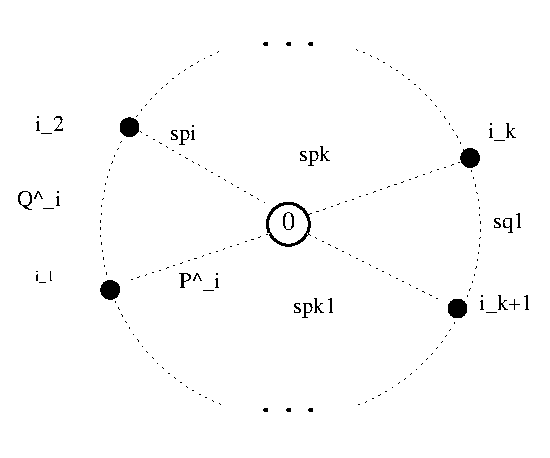
\includegraphics{policy/figures/lemdw.eps}}
\end{psfrags}
\caption{Dispute wheel construction for Lemma~\ref{lem:dwperm}.}
\label{fig:dwperm}
\end{figure}

\begin{proof}
Refer to Figure~\ref{fig:dwperm}. The key idea of the
proof is that, since $\period_i(\sigma) = \period(\sigma)$, we can
repeatedly apply $\sigma$ to the paths $\hat{Q}_i$ and $\hat{P}_i$ and
apply permutation invariance to construct a $\pi$-accepted routing
system with a dispute wheel.

Let $m = \period(\sigma)$.  Define the sequence $i_1, i_2,
\ldots, i_m$ by $i_k = \sigma^{k-1}(i)$ for $k = 1,\ldots,m$.  
Since $\period(\sigma) = \period_i(\sigma)$, the nodes
$i_1,\ldots,i_m$ are all distinct.  For $k = 1,\ldots,m$, define
$\prec_{i_k} = \sigma^{k-1}(\prec_i)$; since the nodes $i_1, \ldots,
i_m$ are all distinct, this assignment of rankings to
nodes is well defined (\ie, no node is assigned two different
rankings).  By permutation
invariance, since $\prec_i$ is $\pi$-accepted, we conclude
$\prec_{i_k}$ is $\pi$-accepted for all $k$.  For all other nodes
$j$, choose any $\pi$-accepted ranking $\prec_j$.  Let
$\F_j = \P_j^N$ for all nodes $j$.

This permutation defines a $\pi$-accepted routing system $(N, \prec_1, \ldots,
\prec_N, \F_1, \ldots, \F_N)$.  We now construct a dispute wheel for
this system.  Define $Q_k = \sigma^{k-1}(\hat{Q}_i)$, and $P_k =
\sigma^{k-1}(\hat{P}_i)$, for $k = 1, \ldots, m$.  We claim that these
definitions yield a dispute wheel.

Since $\F_j = \P_j^N$ for all $j$, all paths are feasible.  Next,
since $\hat{Q}_i$ is a path from $i_1 = i$ to $i_2 = \sigma(i)$, we conclude
that $Q_k$ is a path from $i_k$ to $i_{k+1}$ for all $k$ (where we
define $i_{m+1} = i_1$).  We now observe that:
\begin{align*}
\sigma^{k-1}(R_i) & = \sigma^{k-1}(i) \sigma^{k-1}(\hat{Q}_i) \sigma^{k}(i)
\sigma^{k}(\hat{P}_i) 0 \\
& = i_k Q_{k} i_{k+1}
P_{k+1} 0.
\end{align*}
Finally, since $\prec_{i_k} = \sigma^{k-1}(\prec_i)$ and $R_i \succ_i
\hat{P}_i$, we have $\sigma^{k-1}(R_i) \succ_{i_k}
\sigma^{k-1}(\hat{P}_i)$.  Using the preceding derivation and the fact
that $P_k = \sigma^{k-1}(\hat{P}_i)$, we conclude that $i_k Q_k
i_{k+1} P_{k+1} 0 \succ_{i_k} i_k P_k 0$, as required.

Thus, we have established that $i_1, \ldots, i_m$, together with
$Q_1, \ldots, Q_m$ and $P_1, \ldots,
P_m$, constitute a dispute wheel.
\end{proof}


The preceding lemma reduces the search for a dispute wheel to a search
for a permutation and a $\pi$-accepted ranking with the
stated properties.  Observe from Equation~\eqref{eq:tailmap} that the permutation
$\sigma$ maps the path $\hat{P}_i$ into the ``tail'' of the path $R_i$;
in applying Lemma~\ref{lem:dwperm}, we will construct a partial
permutation by mapping a path $\hat{P}_i$ into the ``tail'' of $R_i$ as
in \eqref{eq:tailmap}, and then we will complete the permutation by
adding nodes to the system if necessary so that $\period_i(\sigma) =
\period(\sigma)$.  We use this approach to prove two theorems; the first
states that if an ARC function accepts at least one ranking
that prefers an $n$-hop path less than a path of at least $n+2$ hops,
then the ARC function is not safe under filtering.

\begin{theorem}
\label{th:unsafe}
Let $\pi$ be an ARC function.  Suppose there exists a node $i$
with $\pi$-accepted ranking $\prec_i$, and two paths $R_i,
\hat{P}_i \in \P_i^N$ such that $\length(R_i) > \length(\hat{P}_i) + 1$
and $R_i \succ_i \hat{P}_i$.  Then, $\pi$ is not safe under filtering.
\end{theorem}



\begin{proof}
The proof relies on Lemma~\ref{lem:dwperm} to build a
dispute wheel.  First, using scale invariance of the ARC function,
we show that the stated conditions of the theorem ensure that there
exist two paths $R_i'$, $\hat{P}_i'$ such that: $\length(R_i') \geq
\length(\hat{P}_i') + 1$; $R_i'$ is more preferred than $\hat{P}_i'$
for some $\pi$-accepted ranking; and $R_i'$ and
$\hat{P}_i'$ have no nodes in common, other than $i$ and $0$.
Lemma~\ref{lem:drperm} then completes the proof of the theorem through
two 
steps: first, once we have found the paths $R_i'$ and $\hat{P}_i'$, we
use them to build a permutation $\sigma$ such that the conditions of
Lemma~\ref{lem:dwperm} are satisfied; and second, we show that the
dispute wheel given by Lemma~\ref{lem:dwperm} is in fact a dispute
ring, by checking that no nodes are repeated around the wheel.

We first construct the paths $R_i'$ and $\hat{P}_i'$ as described in
the previous paragraph.  Let $i$, $\prec_i$, $R_i$, and $\hat{P}_i$ be
given as in the theorem.  Let $\ell = \length(\hat{P}_i)$; \ie,
$\hat{P}_i = i u_1 u_2 \ldots u_{\ell-1} 0$.  We add $\ell$ new nodes
to the routing system, and label them $v_1, \ldots, v_\ell$; let $N' =
N + \ell$.  By scale invariance, there exists a $\pi$-accepted
ranking $\prec_i^{N'}$ on the set of paths $\P_i^{N'}$
with $\prec_i$ as a subranking.  For such a ranking
$\prec_i^{N'}$ we have $R_i \succ_i^{N'} \hat{P}_i$.

But now consider the path $T_i = i v_1 \ldots v_\ell 0$; note that
$\length(T_i) = \ell+1$.  Since $R_i
\succ_i^{N'} \hat{P}_i$, either $T_i \succ_i^{N'} \hat{P}_i$, or $R_i
\succ_i^{N'} T_i$.  In the former case, let $R_i' = T_i$, $\hat{P}_i'
= \hat{P}_i$; and in the latter case, let $R_i' = R_i$, and
$\hat{P}_i' = T_i$.  Then $\length(R_i') \geq \length(\hat{P}_i') + 1$,
$R_i' \succ_i^{N'} \hat{P}_i'$, and $R_i'$ and $\hat{P}_i'$ have no
nodes in common other than $i$ and $0$.

The following lemma uses Lemma~\ref{lem:dwperm} to construct a dispute wheel.

\begin{lemma}
\label{lem:drperm}
Let $\pi$ be an ARC function.  Suppose there exists a node $i$
with $\pi$-accepted ranking $\prec_i$ over $\P_i^N$, and
two paths $R_i, \hat{P}_i
\in \P_i^N$ such that:
\begin{enumerate}
\itemsep=-1pt
\item $\length(R_i) \geq \length(\hat{P}_i) + 1$;\\
\item $R_i \succ_i \hat{P}_i$; and\\
\item $R_i$ and $\hat{P}_i$ have no nodes in common other than $i$ and
$0$.
\end{enumerate}
Then there exists a $\pi$-accepted routing system for which there exists a
dispute ring.
\end{lemma}

{\em Proof of Lemma}.  The proof of this lemma proceeds by using scale
invariance: we add enough new nodes to the system to allow us to build
a permutation such that the conditions of Lemma~\ref{lem:dwperm} are
satisfied.  The key insight is that we initially construct the
permutation $\sigma$ by
mapping the path $\hat{P}_i$ into the ``tail'' of the path $R_i$.  We
then add enough nodes so that when we complete the definition of
$\sigma$, we have $\period_i(\sigma) = \period(\sigma)$.

Let $\length(\hat{P}_i) = n$, and let $h = \length(R_i) -
n$; note that, by Condition~1 in the statement of the lemma, we know $h
\geq 1$. 
Define $i_1 = i$.  We label the nodes so that $\hat{P}_i = i_1 i_2
\ldots i_n 0$, and $R_i = i_1 x_1 x_2 \ldots x_{h-1} \hat{i}_1
\hat{i}_2 \ldots \hat{i}_n 0$.  We want to define a permutation
$\sigma$ that will map the path $i_1
\ldots i_n 0$ to the tail of $R_i$, \ie, to the path $\hat{i}_1
\ldots \hat{i}_n 0$.  However, this does not completely define a
permutation, so we must add additional nodes to ensure that
$\period_i(\sigma) = \period(\sigma)$.

We add $2(h-1) + n$
additional nodes to the system, labeled $\hat{x}_1, \ldots,
\hat{x}_{h-1}$, and $i'_1,\ldots,i'_n,x'_1,\ldots,x'_{h-1}$.  By scale
invariance, we know there exists at least one $\pi$-accepted
ranking $\hat{\prec}_i$ over all paths using this larger
set of nodes, such that $\hat{\prec}_i$ has $\prec_i$ as a
subranking.  In particular, since $R_i \succ_i \hat{P}_i$, we have
$R_i \hat{\succ}_i \hat{P}_i$.  We now define a permutation
$\sigma$ according to the following maps:
\begin{align*}
i_k & \to \hat{i}_k \to i'_k \to i_k,\quad k = 1,\ldots,n;\\
x_k & \to \hat{x}_k \to x'_k \to x_k,\quad k = 1,\ldots,h-1.
\end{align*}
That is, $\sigma(i_k) = \hat{i_k}$, $\sigma(\hat{i_k}) = i'_k$, etc.
For all nodes $j$ not listed, we define $\sigma(j) = j$.  Note that
the period of $\sigma$ is $\period(\sigma) = 3$, and of course
$\period_i(\sigma) = \period_{i_1}(\sigma) = 3 = \period(\sigma)$.  
Finally, note that by definition of $\sigma$, we have $R_i = i \hat{Q}_i
\sigma(i) \sigma(\hat{P}_i) 0$, where $\hat{Q}_i = i x_1 \ldots
x_{h-1} \hat{i}_1$.

\begin{figure}
\centering
\begin{psfrags}
%\epsfig{file=figures/lemdr.eps,width=0.25\textwidth}
%
\psfrag{0}{$0$}
\psfrag{i_1}{$i_1$}
\psfrag{i_n}{$i_n$}
\psfrag{i'_1}{$i'_1$}
\psfrag{i'_n}{$i'_n$}
\psfrag{i^_1}{$\hat{i}_1$}
\psfrag{i^_n}{$\hat{i}_n$}
%
\psfrag{x_1}{$x_1$}
\psfrag{x_h-1}{$x_{h-1}$}
\psfrag{x'_1}{$x'_1$}
\psfrag{x'_h-1}{$x'_{h-1}$}
\psfrag{x^_1}{$\hat{x}_1$}
\psfrag{x^_h-1}{$\hat{x}_{h-1}$}
\resizebox{0.45\textwidth}{!}{\includegraphics{policy/figures/lemdr.eps}}
\end{psfrags}
\caption{Dispute ring construction for Lemma~\ref{lem:drperm}.}
\label{fig:lemdr}
\end{figure}

Thus, the conditions of Lemma~\ref{lem:dwperm} have been satisfied by
the ranking $\hat{\prec}_i$, the paths $R_i$ and
$\hat{P}_i$, and the permutation $\sigma$; so we know there exists a
$\pi$-accepted routing system for which there exists a 
dispute wheel.  To complete the proof, we need only check that
the dispute wheel is a dispute ring.  Note that the wheel has three
pivot nodes.  Furthermore, to check that no nodes are repeated around
the wheel, we simply enumerate the elements of our dispute wheel:
%\begin{align*}
$\hat{Q}_i = i_1 x_1 \ldots x_{m-1} \hat{i}_1$;
$\sigma(\hat{Q}_i) = \hat{i}_1 \hat{x}_1 \ldots \hat{x}_{m-1} i_1'$;
$\sigma^2(\hat{Q}_i) = i_1' x'_1 \ldots x'_{m-1} i_1$ ;
$\hat{P}_i = i_1 \ldots i_n 0$;
$\sigma(\hat{P}_i) = \hat{i}_1 \ldots \hat{i}_n 0$; and
$\sigma^2(\hat{P}_i) = i'_1 \ldots i'_n 0$.
%\end{align*}
It is straightforward to check that these paths constitute a dispute
ring: in Figure~\ref{fig:lemdr}, note that the dispute
wheel constructed from these paths has no repeated
nodes.\hfill$\blacksquare$\\ 

Lemma~\ref{lem:drperm} completes the proof of the theorem: we have shown
that if some $\pi$-accepted ranking exists satisfying the
conditions of the theorem, then using only permutation invariance and
scale invariance we can build a $\pi$-accepted routing system with a
dispute ring.  This routing system is then unsafe under filtering,
by Proposition~\ref{prop:drsafety}.
\end{proof}

The preceding theorem suggests that ARC functions that are safe under
filtering are closely related to the shortest hop count ARC function,
because no rankings can be accepted where $n$ hop paths are
less preferred than ($n+k$)-hop paths, for $k\geq 2$.  The next theorem
draws this relationship even closer, by proving that there exists a
dispute wheel if an ARC function accepts any ranking
where an $n$-hop path is less preferred than an ($n+1$)-hop path.

\begin{theorem}
\label{th:dw}
Let $\pi$ be an ARC function.  Suppose there exists a node $i$
with $\pi$-accepted ranking $\prec_i$, and two paths $R_i,
\hat{P}_i \in \P_i^N$ such that $\length(R_i) = \length(\hat{P}_i) + 1$
and $R_i \succ_i \hat{P}_i$.  Then there exists a $\pi$-accepted
routing system with a dispute wheel.
\end{theorem}


\begin{proof}
As in the proof of Lemma \ref{lem:drperm}, our basic
approach is to map the path $\hat{P}_i$ into the ``tail'' of the path
$R_i$.  This partially defines a permutation $\sigma$.  Using a graphical
approach, we show how to add nodes to the system and
complete the 
permutation $\sigma$ so that $\period_i(\sigma) = \period(\sigma)$.
We then apply Lemma \ref{lem:dwperm} to conclude
there exists a $\pi$-accepted routing system with a dispute wheel.

To begin, write $R_i = i i_1 \ldots i_n
0$, and $\hat{P}_i = i v_1
\ldots v_{n-1} 0$.  We will partially define a permutation $\sigma$,
and then add nodes and ``complete'' the permutation so that $\sigma$
satisfies the conditions of Lemma \ref{lem:dwperm}.  For all
nodes $j \not\in R_i \union \hat{P}_i$, we define $\sigma(j) = j$.
Let $V = R_i \union \hat{P}_i \setminus \{ 0\} = \{ i, i_1, \ldots, i_n, v_1, \ldots,
v_{n-1}\}$; \ie, $V$ is the set of the nonzero nodes in $R_i \union \hat{P}_i$.  We
define a {\em directed} graph on the vertex set $V$, by defining the set of arcs $A$
as follows: $A = \{ (i, i_1)\} \union \{ (v_k, i_{k+1}) : k = 1,\ldots,n-1
\}$.  Define the graph $G = (V,A)$.

We can immediately make the following observations about $G$: (1) each
node in $V$ has either exactly one outgoing link and no incoming
links; or exactly one incoming link and no outgoing links; or exactly
one incoming link and exactly one outgoing link; and (2) from the
definition of $A$, node $i$ has exactly one outgoing link and no
incoming links.  We interpret the graph $G$ as a partial
representation of the permutation $\sigma$, by defining $\sigma(j) =
k$ if $(j,k) \in A$.

Of course, this only partially defines $\sigma$, and we now consider
how we should complete the definition of $\sigma$.  Let $T_1, \ldots T_m$ be the
disjoint connected components of $G$; we write $T_k = (V_k, A_k)$.  By
the definition of ``connected component'', we know $V_k \cap V_{k'} = A_k \cap A_{k'} =
\emptyset$ for $k \neq k'$.  We assume without loss of generality that
$i \in V_1$.

Our approach is to first define $\sigma$ for all the nodes in each
connected component $T_k$, for $k = 2,\ldots,m$.  From the
observations above, we can enumerate the nodes in $V_k$ as $V_k = \{
u_1, u_2, \ldots, u_\ell\}$, such that each $u_r$ has a link to 
$u_{r+1}$, for $r = 1,\ldots,\ell-1$; and either $u_\ell$ has no
outgoing links (in which case $T_k$ is just a ``segment'') or $u_\ell$ has
a link to $u_1$ (in which case $T_k$ is a ``cycle'').  We define
$\sigma(u_r) = u_{r+1}$, where we interpret $u_{\ell+1}$ as $u_1$.  Thus, in a
segment or cycle, each node is mapped to its successor; in addition, in a
segment, the last node is mapped to the first node.  This defines the
permutation $\sigma$ for all nodes, except those in $V_1$.

To complete the proof, we will add enough nodes and extend the
definition of $\sigma$ so that $\period_i(\sigma) = \period(\sigma)$;
we can then apply Lemma \ref{lem:dwperm}.  Note that for all nodes $j \in V_2
\cup \cdots \cup V_m$, we can compute $\period_j(\sigma)$ based on the
preceding definition.  Let $K$ be the least common multiple of
$\period_j(\sigma)$, over all $j \in V_2 \cup \cdots \cup V_m$.  We
then {\em add} nodes to the system, and in particular to the set
$V_1$, until $|V_1|$ (\ie, the number of nodes in $V_1$) is a
{\em multiple} of $K$.  Let the nodes added be $z_1, \ldots, z_s$;
these nodes will eventually become the pivots of the dispute wheel.  We
know that $A_1$ must be of the form $\{ (i,i_1), (i_1, u_1),\ldots, (u_{\ell-1},
u_\ell)\}$ for some nodes $u_1, \ldots, u_\ell \in V$.  We define
$\sigma$ as follows: $\sigma(i) = i_1$; $\sigma(i_1) = u_1$;
$\sigma(u_r) = u_{r+1}$, for $r = 1,\ldots,\ell-1$; $\sigma(u_\ell) =
z_1$; $\sigma(z_r) = z_{r+1}$, for $1 \leq r \leq s-1$; and
$\sigma(z_s) = i$.  Thus, it is as if we added the nodes $z_1, \ldots,
z_s$, and turned the segment $T_1$ into a cycle.  Since the length of
this cycle is a multiple of $K$, it is clear that $\period(\sigma)$ is
a multiple of $K$, and $\period_i(\sigma) = \period(\sigma)$.  

By scale invariance, even though we have added nodes to the system, we
can extend $\prec_i$ to a $\pi$-accepted ranking over the
resulting larger set of paths, while maintaining the preference of
$R_i$ over $\hat{P}_i$ for node $i$.  Furthermore, recalling our initial
definition 
of the arc set $A$, it is clear that we have $R_i = i i_1 \ldots i_n 0
= i \sigma(i) \sigma(v_1) \ldots \sigma(v_{n-1}) 0 = i \sigma(i)
\sigma(\hat{P}_i) 0$.  Thus, we can apply Lemma \ref{lem:dwperm}, with
$\hat{Q}_i = \emptyset$, to
conclude there exists a $\pi$-accepted routing system with a dispute
wheel.
\end{proof}

The preceding results should not be interpreted as suggesting that we
cannot find a routing system that is safe under filtering, where
nodes prefer ($n+k$)-hop paths over $n$-hop paths.  Indeed, 
from Figure~\ref{fig:dw_no_osc}, there are routing systems where nodes prefer
$3$-hop paths over $1$-hop paths, and yet the system is safe under
filtering.  However, checking whether such systems are safe under
filtering requires global verification; the theorems we have presented
suggest that safety under filtering cannot be guaranteed through local
verification alone, if some nodes are allowed to prefer ($n+k$)-hop
paths over $n$-hop paths.

Furthermore, the two results in this section highlight the importance of
dispute rings.  Theorem \ref{th:unsafe} gives the
strong result that an ARC function that allows some ($n+k$)-hop path to be
more preferred than an $n$-hop path cannot guarantee safety under
filtering, if $k \geq 2$.  Theorem \ref{th:dw} only
guarantees the existence of a dispute wheel if an ARC function that allows some
($n+1$)-hop path to be more preferred than an $n$-hop path---we
cannot draw conclusions regarding the stability or safety of a routing
system on the basis of the existence of a dispute wheel (see
Figure~\ref{fig:dw_no_osc}).  

% be misinterpreted as suggesting that Nevertheless, the
% class of ARC functions that are safe under filtering is
% {\em strictly larger} than just the singleton consisting of the
% shortest hop count RC function.  That is, there {\em do} exist ARC
% functions that guarantee safety under filtering, and where an $n+1$
% hop path can be more preferred than an $n$ hop path.  This is the
% content of the following example.


% \begin{example}
% We define a ARC function $\pi$ as follows.  For each node $i$, a
% ranking $\prec_i$ over $\P_i^N$ is accepted if it satisfies the
% following conditions:
% \begin{enumerate}
% \item If $N < 5$, then $\prec_i$ is a 
% shortest hop count ranking; \ie, if $\length(P_i) <
% \length(\hat{P}_i)$ implies $P_i \succ_i \hat{P}_i$ for all $P_i,
% \hat{P}_i \in \P_i^N$.
% \item If $N \geq 5$, then there exist nodes $i_1, i_2, i_3, i_4$ and
% paths $\hat{P}_i^0 = i i_1 i_2 i_3 i_4 0$, $P_i^0 = i i_3 i_4 i_2 0$
% such that $\hat{P}_i^0 \succ_i^N P_i^0$.  For all other pairs of paths $P_i,
% \hat{P}_i \in \P_i^N$, there holds $P_i \succ_i \hat{P}_i$ if $\length(P_i) <
% \length(\hat{P}_i)$, as long as either $P_i \neq P_i^0$ or $\hat{P}_i^0$
% \end{enumerate}
% Thus for $N \geq 5$, $\prec_i$ is essentially a shortest hop count
% ranking, except that exactly {\em one} 5 hop path is
% allowed to be preferred over one 4 hop path.  

% We claim that this ARC function is safe under filtering.  Suppose
% not, and let $(N, \prec_1,\ldots, \prec_N, \F_1, \ldots, \F_N)$ be a
% $\pi$-accepted routing system which is not safe under filtering. By
% Proposition \ref{}, there exists a dispute wheel for this system,
% given by nodes $i_1, \ldots, i_m$, together with paths $Q_{i_1},
% \ldots, Q_{i_m}$, and $P_{i_1}, \ldots, P_{i_m}$.  Given the structure
% of the rankings accepted by $\pi$, it is not difficult
% to check that in this dispute wheel, it must be the case that
% $P_{i_k}$ is a 4 hop path for each $k$, and $Q_{i_k}$ is a one hop
% path (a single link).

% Consider just the nodes $i_m$, $i_1$, and $i_2$.  We write $P_{i_1} =
% i_1 j_2 j_3 j_4 0$; since $Q_{i_m}$ is a one hop path, we have
% $Q_{i_m} = i_m i_1$.  Now given that $\prec_{i_m}$ is $\pi$-accepted,
% it must be the case from the definition of $\pi$ above that $P_{i_m} = 



% \Given $N$, let $\prec_1$
% be a ranking for node $1$ that satisfies the following 

% Consider a $5$-node BGP system whereby node $1$'s rankings are as
% follows:
% \begin{enumerate}
% \itemsep=-1pt
% \item All paths shorter than $4$ hops.
% \item All $4$-hop paths other than path $(1 4 5 3 0)$.
% \item The $5$-hop path $(1 2 3 4 5 0)$.
% \item The $4$-hop path $(1 4 5 3 0)$.
% \item All $5$-hop paths other than $(1 2 3 4 5 0)$.
% \item All paths longer than $5$ hops.
% \end{enumerate}
% Suppose that nodes $2 \ldots 5$ have a set of rankings dictated by
% the permutation $\sigma(1) = 2, \sigma(2) = 1, \sigma(3) = 5, \sigma(4)
% = 3, \sigma(5) = 4$.  If we apply this permutation once, then node $2$
% prefers one $5$-hop path over one $4$-hop path (\ie, $(2 1 5 4 3 0)
% \prec_2^5 (2 3 4 5 0)$).  These two sets of rankings create the set
% of rankings depicted in Figure~\ref{fig:allow_one}.  Since each node
% is only permitted to prefer one $N+1$-hop path over an $N$-hop path,
% then it is clear that the arc $Q_1 P_*$ must be no more than $4$ hops.
% This, however, implies that the existence of a dispute wheel would
% require node $*$ to prefer the path $(* 1 4 5 3 0)$, a $6$-hop path over
% $P_*$, a path of $3$ or fewer hops, which $\pi$ does not accept.
% Therefore, $\pi$ can allow one such path of length $N+1$ over $N$
% without inducing a dispute wheel.
% \end{example}

% % \begin{defn}[Order preserving]
% % A pair of paths $P_i$ and $\hat{P}_i$ is {\em order preserving} if, for
% % any two nodes $j,k \in P_i \cap \hat{P}_i$, either $j$ is further than
% % $k$ from $0$ or $k$ is further than $j$ from $0$ for {\em both} $P_i$
% % and $\hat{P}_i$.
% % \end{defn}

% \begin{defn}[Order preserving]
% Given a pair of paths $P_i, \hat{P}_i \in \P_i^N$, we say $\hat{P}_i$
% is {\em order preserving} with respect to $P_i$ if
% $\hat{P}_i$ can be derived from $P_i$ by removing nodes from $P_i$.
% That is, if $P_i = i i_1 i_2 \ldots i_n 0$, then $\hat{P}_i = i
% i_{k_1} \ldots i_{k_m} 0$, for some sequence $1 \leq k_1 < k_2 <
% \ldots < k_m \leq n$.
% \end{defn}

% \begin{prop}
% Let $\pi$ be a ARC function.  Suppose we are given a node $i$
% with $\pi$-accepted ranking $\prec_i$, and two paths $P_i, \hat{P}_i
% \in \P_i^N$ such that: (1) $\hat{P}_i$ is order preserving with respect to
% $P_i$; (2) $length(P_i) = length(\hat{P}_i) + 1$; and (3) $P_i
% \succ_i \hat{P}_i$.  Then there exists a $\pi$-accepted BGP system
% such that there exists a dispute wheel.
% \end{prop}

% {\em Proof}. Note that $\hat{P}_i$ is simply $P_i$ with a single node removed.  We
% write $P_i = i i_1 \ldots i_n 0$, and suppose $\hat{P}_i = i i_1
% \ldots i_{k-1} i_{k+1} \ldots i_n 0$; \ie, $\hat{P}_i$ is identical
% to $P_i$ with node $i_k$ removed from the path.  Define the
% permutation $\sigma$ as follows:
% \begin{align*}
% \sigma(i) & = i_1; \\
% \sigma(i_\ell) & = i_{\ell+1},\quad 1 \leq \ell \leq k-1;\\
% \sigma(i_\ell) & = i_\ell,\quad k+1 \leq \ell \leq n;\\
% \sigma(i_k) &= i.
% \end{align*}

% We now check that the conditions of Lemma \ref{lem:dwperm} are
% satisfied.  By assumption, $\prec_i$ is $\pi$-accepted, and $P_i
% \succ_i \hat{P}_i$.  We now show that $\period(\sigma) =
% \period_i(\sigma)$.  To see this, let $S = \{ i, i_1, \ldots, i_k
% \}$.  Note that $\sigma$ is the identity map for all nodes not in $S$,
% and $\sigma$ is a cyclic permutation on the $k+1$ nodes in $S$.  Thus
% $\period_i(\sigma) = \period(\sigma) = k+1$.  Finally, let $Q_i = i
% i_1$.  Then observe that by definition $\sigma(\hat{P}_i) = i_1
% \ldots i_n 0$ and $\sigma(i) = i_1$, so that $P_i = i Q_i \sigma(i)
% \sigma(\hat{P}_i) 0$, as required.  Applying Lemma \ref{lem:dwperm},
% we conclude there exists a $\pi$-accepted BGP system with a dispute
% wheel.\hfill$\blacksquare$\\


